\subsection{UC19 - Richiesta di spostamento}
\begin{figure}[H]
  \centering
  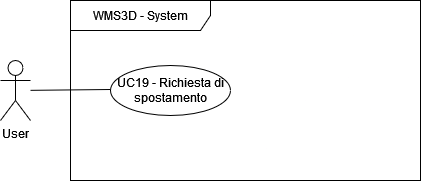
\includegraphics[width=0.8\textwidth]{UC_diagrams_11-20/UC19_sys.drawio.png}
   \caption{Diagramma UML UC19}
\end{figure}
\begin{figure}[H]
  \centering
  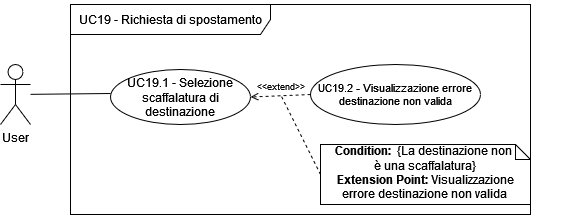
\includegraphics[width=0.8\textwidth]{UC_diagrams_11-20/UC19.drawio.png}
   \caption{Diagramma UML UC19 - dettaglio}
\end{figure}
\begin{itemize}
    \item \textbf{Attori:} User.
    \item \textbf{Pre-condizione:} L'utente ha selezionato un prodotto [UC15] che è stato posizionato [UC14].
    \item \textbf{Post-condizione:} L'utente richiede lo spostamento del prodotto.
    \item \textbf{Scenario Principale:} L'utente seleziona la destinazione per la movimentazione del prodotto [UC19.1] e si richiede lo spostamento.  
    \item \textbf{Generalizzazioni:} -
    \item \textbf{Estensioni:} -
\end{itemize}


\subsubsection{UC19.1 - Selezione scaffalatura di destinazione}
\begin{figure}[H]
  \centering
  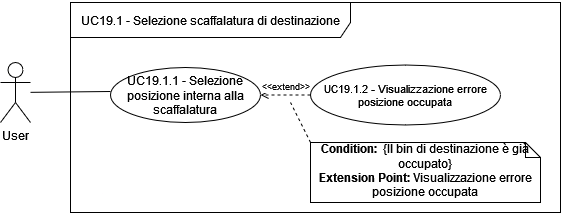
\includegraphics[width=0.8\textwidth]{UC_diagrams_11-20/UC19.1.drawio.png}
   \caption{Diagramma UML UC19.1}
\end{figure}
\begin{itemize}
    \item \textbf{Attori:} User.
    \item \textbf{Pre-condizione:} L'utente vuole richiedere lo spostamento di un prodotto [UC19].
    \item \textbf{Post-condizione:} Viene selezionata la destinazione dello spostamento.
    \item \textbf{Scenario Principale:} L'utente seleziona la scaffalatura, e in particolar modo il bin\textsuperscript{G} [UC19.1.1], di destinazione della movimentazione del prodotto.
    \item \textbf{Generalizzazioni:} -
    \item \textbf{Estensioni:} È presente una estensione:
    \begin{itemize}
        \item UC19.2 - Visualizzazione errore destinazione non valida.
    \end{itemize}
\end{itemize}


\paragraph{UC19.1.1 - Selezione posizione interna alla scaffalatura}
\begin{itemize}
    \item \textbf{Attori:} User.
    \item \textbf{Pre-condizione:}  L'utente vuole richiedere lo spostamento di un prodotto [UC19].
    \item \textbf{Post-condizione:} Viene selezionato il bin\textsuperscript{G} interno alla scaffalatura come destinazione dello spostamento.
    \item \textbf{Scenario Principale:} L'utente dopo aver creato un prodotto sceglie a quale bin\textsuperscript{G} destinare il prodotto.
    \item \textbf{Generalizzazioni:} -
    \item \textbf{Estensioni:} È presente una estensione nel caso in cui il bin\textsuperscript{G} scelto sia occupato:
    \begin{itemize}
        \item UC19.1.2- Visualizzazione errore posizione occupata.
    \end{itemize}
\end{itemize}


\paragraph{UC19.1.2 - Visualizzazione errore posizione occupata}
\begin{itemize}
    \item \textbf{Attori:} User.
    \item \textbf{Pre-condizione:}  L'utente cerca di destinare lo spostamento del prodotto ad un bin già occupato da un altro prodotto.
    \item \textbf{Post-condizione:} L'utente visualizza un messaggio d'errore e la richiesta non viene inoltrata.
    \item \textbf{Scenario Principale:} L'utente visualizza un messaggio informativo sull'errore. L'utente dovrà cambiare destinazione.
    \item \textbf{Generalizzazioni:} -
    \item \textbf{Estensioni:} -
\end{itemize}


\subsubsection{UC19.2 - Visualizzazione errore destinazione non valida}
\begin{itemize}
    \item \textbf{Attori:} User.
    \item \textbf{Pre-condizione:}  L'utente cerca di destinare il prodotto in una posizione al di fuori delle scaffalature.
    \item \textbf{Post-condizione:} L'utente visualizza un messaggio d'errore e il posizionamento non viene permesso.
    \item \textbf{Scenario Principale:} L'utente visualizza un messaggio informativo sull'errore. L'utente dovrà cambiare destinazione.
    \item \textbf{Generalizzazioni:} -
    \item \textbf{Estensioni:} -
\end{itemize}